%%%%%%%%%%%%%%%%%%%%%%%%%%%%%%%%%%%%%%%%%%%%%%%%%%%%%%%%%%%%%%%%%%%%%%
% Lớp 10 | Xác suất | Xác suất của biến cố
% Dạng 0D0?2-6: Liên quan hình học
% Số câu: 6  (sinh tự động bởi tach_cau.py; từ nay thầy sửa trực tiếp file này)
%%%%%%%%%%%%%%%%%%%%%%%%%%%%%%%%%%%%%%%%%%%%%%%%%%%%%%%%%%%%%%%%%%%%%%

%%%%%%%%%%%%%%%% TRẮC NGHIỆM 4 PHƯƠNG ÁN %%%%%%%%%%%%%%%%

% nguồn: MaHoaNH_TracNghiem_Lop10
\begin{ex}%[0D0H2-6]%[ma:a7dd5f91]
	Cho đa giác đều có $100$ đỉnh. Chọn ngẫu nhiên $3$ đỉnh. Tính xác suất để $3$ đỉnh được chọn là $3$  đỉnh của một tam giác tù.
	 \choice
		 {$\dfrac{18}{25}$}
		 {$\dfrac{7}{25}$}
		{$\dfrac{3}{11}$} 
		{\True $\dfrac{8}{11}$} 
	\loigiai{ 
		\begin{center}
			\begin{tikzpicture}[scale=1,>=stealth,font=\footnotesize,line join=round,line cap=round]
					\def\r{2.5} \def\g  {36}
					 \path
						(0,0) coordinate (O) 
					\foreach \i in {0,1,2,...,9}{(\i*\g:\r)  coordinate (A\i)};
					 \draw (O) circle (\r);
					\draw (A0)--(A1)--(A2)--(A3)--(A4)--(A5)--(A6)--(A7)--(A8)--(A9)--cycle; 
					 \draw [fill=cyan!50] (A5)--(A3)--(A1)--cycle (A0)--(A5);
					\node[left] at  (A5){$A$};
					 \node[right] at (A0){$A'$};
					\node[above right] at (A1){$C$}; 
					\node[above] at (A3){$B$}; 
					 \node[below] at (O){$O$};
					\draw pic[draw,angle  radius=4mm]{angle=A5--A3--A1};
					 \foreach \x in {O,A0,A1,A2,A3,A4,A5,A6,A7,A8,A9}{\fill[black] (\x) circle (1.5pt);}
				\end{tikzpicture}
		\end{center}
		Số phần tử của không gian mẫu là  $\mathrm{C}_{100}^3$.\\
		Gọi đường tròn $(O)$ là đường tròn ngoại tiếp đa giác. Xét $A$ là $1$ đỉnh bất kỳ của đa giác,kẻ đường kính $AA'$ thì $A'$ cũng là $1$ đỉnh của đa giác. Đường kính $AA'$ chia $(O)$ thành $2$ nửa đường tròn, với mỗi cách chọn ra $2$  điểm $B$ và $C$ là $2$ đỉnh của đa giác và cùng thuộc $1$ nửa đường tròn, ta được $1$ tam giác tù $ABC$. Khi đó số cách chọn $B$ và $C$ là $2\cdot\mathrm{C}_{49}^2$.\\
		Đa giác có $100$ đỉnh nên số đường chéo là đường kính của đường tròn ngoại tiếp đa  giác là $50$.\\
		Do đó, số  cách chọn ra $3$ đỉnh để lập thành $1$ tam giác tù là $50\cdot2\cdot\mathrm{C}_{49}^2$.\\
		Do đó xác suất cần  tính là $\dfrac{50\cdot2\cdot\mathrm{C}_{49}^2}{\mathrm{C}_{100}^3}=\dfrac{8}{11}$.
	 }
\end{ex}

% nguồn: MaHoaNH_TracNghiem_Lop10
\begin{ex}%[0D0V2-6]%[ma:4c92871b]
	Một đa giác đều $18$ đỉnh nội tiếp trong một đường tròn tâm $O$. Gọi $X$ là tập hợp tất cả các tam giác có  các đỉnh là các đỉnh của đa giác trên. Tính xác suất $\mathrm{P}$ để chọn được một tam giác từ tập $X$ là tam giác cân nhưng không phải tam giác đều.
	\choice 
		{$\mathrm{P}=\dfrac{144}{136}$} 
		 {$\mathrm{P}=\dfrac{7}{816}$}
		 {\True $\mathrm{P}=\dfrac{23}{136}$}
		{$\mathrm{P}=\dfrac{21}{136}$} 
	 \loigiai{
		Số phần tử của  không gian mẫu là $n(X)=\mathrm{C}_{18}^3$.\\
		Ký hiệu đa giác là $A_1 A_2\ldots A_{18}$ nội  tiếp đường tròn $(O)$.\\
		Xét đường kính $A_1 A_{10}$  khi đó số tam giác cân có đỉnh cân là $A_1$ hoặc $A_{10}$ là $2\cdot 8=16$ (tam giác cân).\\
		Mà có tất cả là $9$ đường kính do vậy số tam giác cân có các đỉnh là đỉnh của đa  giác là $9\cdot16=144$ (tam giác cân).\\
		Ta  lại có số tam giác đều có các đỉnh là đỉnh của đa giác đều $18$ đỉnh là $6$.\\
		Vậy xác  suất $\mathrm{P}$ để chọn được một tam giác từ tập $X$ là tam giác cân nhưng không phải tam giác đều là $\mathrm{P}=\dfrac{144-6}{C_{18}^3}=\dfrac{23}{136}$.
	} 
\end{ex}


%%%%%%%%%%%%%%%% ĐÚNG/SAI %%%%%%%%%%%%%%%%

% nguồn: MaHoaNH_DungSai_Lop10
\begin{ex}%[0D0V2-6]%[ma:94c22893]
	Cho đa giác đều $12$ đỉnh. Chọn ngẫu nhiên $3$ đỉnh trong số $12$ đỉnh của đa giác. Xác suất để $3$ đỉnh được chọn tạo  thành tam giác đều là
	\choiceTF 
		{$P=\dfrac{1}{14}$} 
		 {$P=\dfrac{1}{220}$}
		 {$P=\dfrac{1}{4}$}
		{\True $P=\dfrac{1}{55}$} 
	\loigiai{ 
		Số phần  tử của không gian mẫu là $n\left( \Omega \right)=\mathrm{C}_{12}^3=220$. \\
		Gọi $A$ là biến cố ``Chọn được $3$  đỉnh tạo thành một tam giác đều''.\\
		Để $3$ đỉnh được chọn tạo thành một tam giác đều thì các đỉnh đó phải nằm ở vị trí cách đều nhau  nên $n(A)=\dfrac{12}{3}=4$.\\
	Vậy xác suất của biến cố $A$  là $\mathrm{P}(A)=\dfrac{4}{220}=\dfrac{1}{55}$.}
\end{ex}


%%%%%%%%%%%%%%%% TRẢ LỜI NGẮN %%%%%%%%%%%%%%%%

% nguồn: MaHoaNH_TraLoiNgan_Lop10
\begin{bt}%[0D0V2-6]%[ma:3e19580e]
	Chọn ngẫu nhiên $3$ đỉnh  trong một đa giác đều có $21$ đỉnh. Tính xác suất để $3$ đỉnh được chọn lập thành một tam giác cân nhưng không phải là tam giác đều (\textit{Kết quả làm tròn đến chữ số thập phân thứ hai sau dấu phẩy}).
	 \shortans{0,14}
	\loigiai{Số phần tử  của không gian mẫu $\mathrm{C}_{21}^3=1\,330$.\\
		Gọi $O$ là tâm đường tròn ngoại tiếp đa giác đều. Xét một đỉnh $A$ bất kỳ của đa giác: Có $10$ cặp đỉnh đối xứng với nhau qua đường thẳng $O A$, hay có  $10$ tam giác cân tại đỉnh $A$. \\Như vậy với mỗi đỉnh của đa giác có $10$ tam giác nhận nó làm đỉnh của tam giác cân.\\
		Số tam giác đều có $3$ đỉnh là các đỉnh của đa giác là $\dfrac{21}{3}=7$ tam  giác.\\
		Trong các tam giác cân đã xác định ở trên có cả tam giác đều, do mọi tam giác đều thì cân tại  $3$ đỉnh nên các tam giác đều được đếm ba lần.\\
		Suy ra số tam giác cân nhưng không phải là tam giác đều có ba đỉnh là ba đỉnh của đa giác đã cho là $10\cdot  21-3\cdot 7=189$.\\
		Vậy xác suất để chọn được một tam  giác cân nhưng không phải là tam giác đều là
		$$ 
		\mathrm{P}(A)=\dfrac{189}{1\,330}=\dfrac{27}{190} \approx 0{,}14 
		$$ 
	 }
\end{bt}

% nguồn: MaHoaNH_TraLoiNgan_Lop10
\begin{bt}%[0D0V2-6]%[ma:033bf0b0]
	Cho đa giác đều $20$ đỉnh $A_1.A_2\ldots A_{20}$ nội tiếp đường tròn tâm $O$. Chọn ngẫu nhiên ba đỉnh của đa giác đó, tính xác  suất để ba đỉnh được chọn là ba đỉnh của một tam giác vuông (làm tròn kết quả đến chữ số thập phân thứ hai).
	 \shortans{0,16}
	\loigiai{ 
		Gọi $A$ là  biến cố \lq\lq ba đỉnh được chọn là ba đỉnh của một tam giác vuông\rq\rq.\\
		Số cách chọn ra một tam giác bất kì là số cách chọn ra $3$ đỉnh trong $20$  đỉnh của đa giác đã cho\\
		Suy ra  $n(\Omega)=\mathrm{C}_{20}^3=1\,140$. \\
		Tam  giác vuông nội tiếp đường tròn có một cạnh là đường kính.\\
		 Chọn ra $2$ đỉnh là đường kính của đường tròn có $10$ cách.\\
		Chọn ra $1$  đỉnh trong $18$ đỉnh còn lại có $18$ cách.\\
		$\Rightarrow  n(A)=10\cdot18=180$.\\
		Vậy $\mathrm{P}(A)=\dfrac{180}{1140}=\dfrac{3}{19} \approx  0{,}16$.
	} 
\end{bt}

% nguồn: MaHoaNH_TraLoiNgan_Lop10
\begin{bt}%[0D0V2-6]%[ma:9294d83d]
	\immini{Một quân vua được đặt trên một ô giữa bàn cờ vua. Mỗi bước di chuyển, quân vua được chuyển sang một ô khác chung cạnh hoặc chung đỉnh với ô đang đứng (xem hình minh họa). Bạn An di  chuyển quân vua ngẫu nhiên $3$ bước. Tính xác suất để sau $3$ bước đi quân
	vua trở về ô xuất phát? Làm tròn  kết quả đến hàng phần trăm.
	 }{
	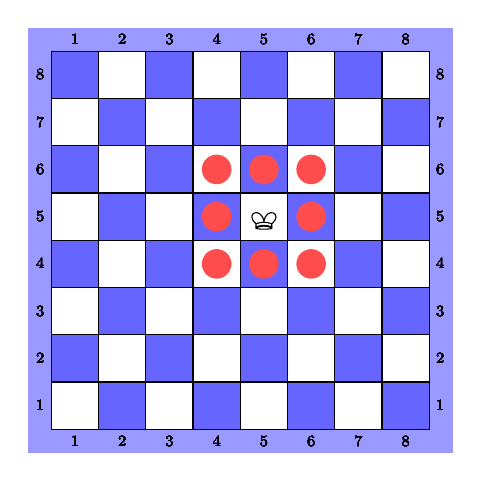
\begin{tikzpicture}[font=\footnotesize,line join=round,line cap=round,>=stealth]
			\begin{scope}[scale=.6]
				\tikzset{vua/.pic={ 
				 \def\a{1}
				 \draw ([shift={(0,-\a/4)}]-\a/2,0)--(-\a/2,0)..controls ++ (140:1) and ++(100:1)..(0,0.15)..controls ++(80:1) and ++(40:1)..(\a/2,0)--++(-90:\a/4)..controls++(-30:0.25) and++(-150:0.25)..(-\a/2,-\a/4);
				 \foreach \d in {0,\a/5,\a/4}{
					\draw[shift={(0,-\d)}](-\a/2,0)--(-\a/2,0)..controls++(20:0.15) and++(180:0.15)..(0,0.1)..controls++(0:0.15)  and++(160:0.15)..(\a/2,0);
					 }}}
					\tikzset{vitri/.pic={ 
				 \def\a{0.75}
				\draw[fill=red!70,draw=none,scale=.5](0,0)  circle (\a/2);
					}} 
				\fill[blue!40](-0.5,-0.5)  rectangle (8.5,8.5);
				\foreach \i in{0,1,...,7} 
				\foreach \j  in{0,1,...,7}
					{ 
				\pgfmathparse{mod (\i+\j,2)?  "blue!60": "white"}
				\fill[\pgfmathresult,draw=black](\i,\j) rectangle (\i+1,\j+1); 
				\pgfmathsetmacro{\k}{int (\j+1)} 
				 \path (0,\j+0.5) node[scale=.7,left]{\k}
					 (8,\j+0.5) node[scale=.7,right]{\k}
					(\j+0.5,0)  node[scale=.7,below]{\k}
					(\j+0.5,8)  node[scale=.7,above]{\k};
				} 
				\path (4.5,4.35)  pic[scale=0.2]{vua};
				\foreach \x/\y in{5/5,4/5,3/5,3/4,3/3,4/3,5/3,5/4} 
				 \path[shift={(0.5,0.5)}](\x,\y) pic{vitri};
			\end{scope}
		\end{tikzpicture}
	} 
	\shortans{0,05} 
	\loigiai{ 
		Gọi $\Omega$ là không gian  mẫu. Từ vị trí của quân vua, cứ mỗi bước sẽ có $8$ vị trí mà quân vua có thể đi. Do đó $|\Omega|=8^3=512$.\\
		Gọi  $A$ là biến cố: \lq\lq sau $3$ bước quân vua về ô xuất phát\rq\rq.
		\begin{itemize}
			\item TH1: đi theo  hình tam giác vuông cân tại đỉnh vua ban đầu $4\cdot 2 = 8$ cách.
			\begin{center}
				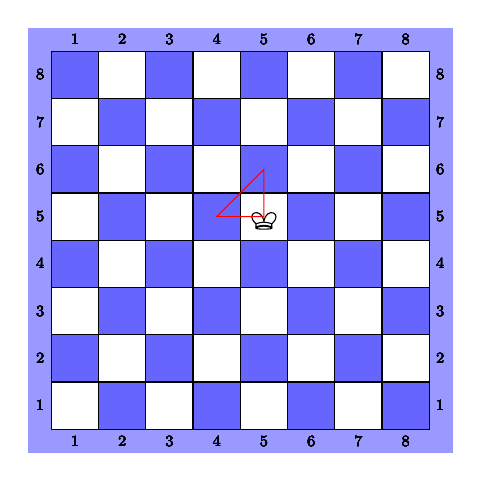
\begin{tikzpicture}[font=\footnotesize,line join=round,line cap=round,>=stealth]
						\begin{scope}[scale=.6]
						\tikzset{vua/.pic={ 
						 \def\a{1}
						\draw ([shift={(0,-\a/4)}]-\a/2,0)--(-\a/2,0)..controls ++  (140:1) and ++(100:1)..(0,0.15)..controls ++(80:1) and ++(40:1)..(\a/2,0)--++(-90:\a/4)..controls++(-30:0.25) and++(-150:0.25)..(-\a/2,-\a/4);
						\foreach \d  in {0,\a/5,\a/4}{
						\draw[shift={(0,-\d)}](-\a/2,0)--(-\a/2,0)..controls++(20:0.15) and++(180:0.15)..(0,0.1)..controls++(0:0.15) and++(160:0.15)..(\a/2,0); 
						}}} 
						 \tikzset{vitri/.pic={
						 \def\a{0.75}
						\draw[fill=red!70,draw=none,scale=.5](0,0) circle  (\a/2);
						 }}
						 \fill[blue!40](-0.5,-0.5) rectangle (8.5,8.5);
						\foreach  \i in{0,1,...,7}
						 \foreach \j in{0,1,...,7}
						{ 
						\pgfmathparse{mod (\i+\j,2)? "blue!60":  "white"}
						\fill[\pgfmathresult,draw=black](\i,\j) rectangle (\i+1,\j+1); 
						\pgfmathsetmacro{\k}{int  (\j+1)}
						\path (0,\j+0.5)  node[scale=.7,left]{\k}
						 (8,\j+0.5) node[scale=.7,right]{\k}
						 (\j+0.5,0) node[scale=.7,below]{\k}
						(\j+0.5,8) node[scale=.7,above]{\k}; 
						} 
						\path (4.5,4.35)  pic[scale=0.2]{vua};
						\draw[color=red] (4.5,4.5)--(4.5,5.5)--(3.5,4.5)--(4.5,4.5); 
						\end{scope}
					\end{tikzpicture}
			\end{center}
			\item TH2: đi theo hình tam giác vuông cân tại đỉnh khác vua có $8\cdot 2= 16$  cách
			\begin{center}
				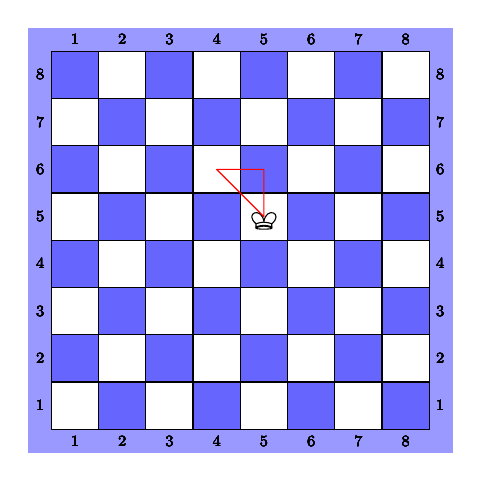
\begin{tikzpicture}[font=\footnotesize,line join=round,line cap=round,>=stealth]
						\begin{scope}[scale=.6]
						 \tikzset{vua/.pic={
						 \def\a{1}
						\draw ([shift={(0,-\a/4)}]-\a/2,0)--(-\a/2,0)..controls ++ (140:1) and ++(100:1)..(0,0.15)..controls ++(80:1) and ++(40:1)..(\a/2,0)--++(-90:\a/4)..controls++(-30:0.25) and++(-150:0.25)..(-\a/2,-\a/4); 
						\foreach \d in {0,\a/5,\a/4}{ 
						 \draw[shift={(0,-\d)}](-\a/2,0)--(-\a/2,0)..controls++(20:0.15) and++(180:0.15)..(0,0.1)..controls++(0:0.15) and++(160:0.15)..(\a/2,0);
						 }}}
						\tikzset{vitri/.pic={ 
						\def\a{0.75} 
						\draw[fill=red!70,draw=none,scale=.5](0,0)  circle (\a/2);
						}} 
						\fill[blue!40](-0.5,-0.5) rectangle  (8.5,8.5);
						\foreach \i  in{0,1,...,7}
						\foreach  \j in{0,1,...,7}
						 {
						\pgfmathparse{mod (\i+\j,2)?  "blue!60": "white"}
						\fill[\pgfmathresult,draw=black](\i,\j) rectangle (\i+1,\j+1); 
						\pgfmathsetmacro{\k}{int  (\j+1)}
						 \path (0,\j+0.5) node[scale=.7,left]{\k}
						(8,\j+0.5)  node[scale=.7,right]{\k}
						(\j+0.5,0)  node[scale=.7,below]{\k}
						(\j+0.5,8) node[scale=.7,above]{\k}; 
						} 
						\path  (4.5,4.35) pic[scale=0.2]{vua};
						\draw[color=red] (4.5,4.5)--(4.5,5.5)--(3.5,5.5)--(4.5,4.5); 
						\end{scope}
					\end{tikzpicture}
			\end{center}
		\end{itemize}
		Do  đó $|A|=8+16=24$ cách.\\
		Xác suất để sau $3$ bước đi quân vua về ô xuất phát  là $$P(A)=\dfrac{|A|}{|\Omega|}=\dfrac{24}{512}=\dfrac{3}{64}.$$
	 }
\end{bt}
